%===================================================================================
\chapter{Code Organization}\label{s:organization}
%===================================================================================

%----------------------------------
\section{SUNDIALS organization}\label{ss:sun_org}
%----------------------------------
% This is a shared SUNDIALS TEX file with description of
% the SUNDIALS organization
%
The family of solvers referred to as {\sundials} consists of the solvers
{\cvode} (for ODE systems), {\kinsol} (for nonlinear algebraic
systems), and {\ida} (for differential-algebraic systems).  In addition,
{\sundials} also includes variants of {\cvode} and {\ida} with sensitivity analysis 
capabilities (using either forward or adjoint methods): {\cvodes} and {\idas},
respectively.

The various solvers of this family share many subordinate modules.
For this reason, it is organized as a family, with a directory
structure that exploits that sharing (see Fig. \ref{f:sunorg}).
\begin{figure}
\subfigure[High-level diagram]
{\centerline{\psfig{figure=sunorg1.eps,width=\textwidth}}}
\subfigure[Directory structure of the source tree]
{\centerline{\psfig{figure=sunorg2.eps,width=\textwidth}}}
\caption {Organization of the SUNDIALS suite}\label{f:sunorg}
\end{figure}
The following is a list of the solver packages presently available:
\begin{itemize}

\item {\cvode},  
  a solver for stiff and nonstiff ODEs $dy/dt = f(t,y)$;

\item {\cvodes},
  a solver for stiff and nonstiff ODEs
  with sensitivity analysis capabilities;

\item {\ida},
  a solver for differential-algebraic systems $F(t,y,y^\prime) = 0$;

\item {\idas},
  a solver for differential-algebraic systems
  with sensitivity analysis capabilities;

\item {\kinsol}, 
  a solver for nonlinear algebraic systems $F(u) = 0$.

\end{itemize}


%----------------------------------
\section{CVODES organization}\label{ss:cvodes_org}
%----------------------------------

\index{CVODES@{\cvodes}!package structure}
The {\cvodes} package is written in ANSI {\CC}. The following
summarizes the basic structure of the package, although knowledge
of this structure is not necessary for its use.

The overall organization of the {\cvodes} package is shown in Figure
\ref{f:cvsorg}.
The basic elements of the structure are a module for
the basic integration algorithm (including forward sensitivity analysis),
a module for adjoint sensitivity analysis, and support for the solution
of nonlinear and linear systems that arise in the case of a stiff system.  
\begin{figure}[!ht]
{\centerline{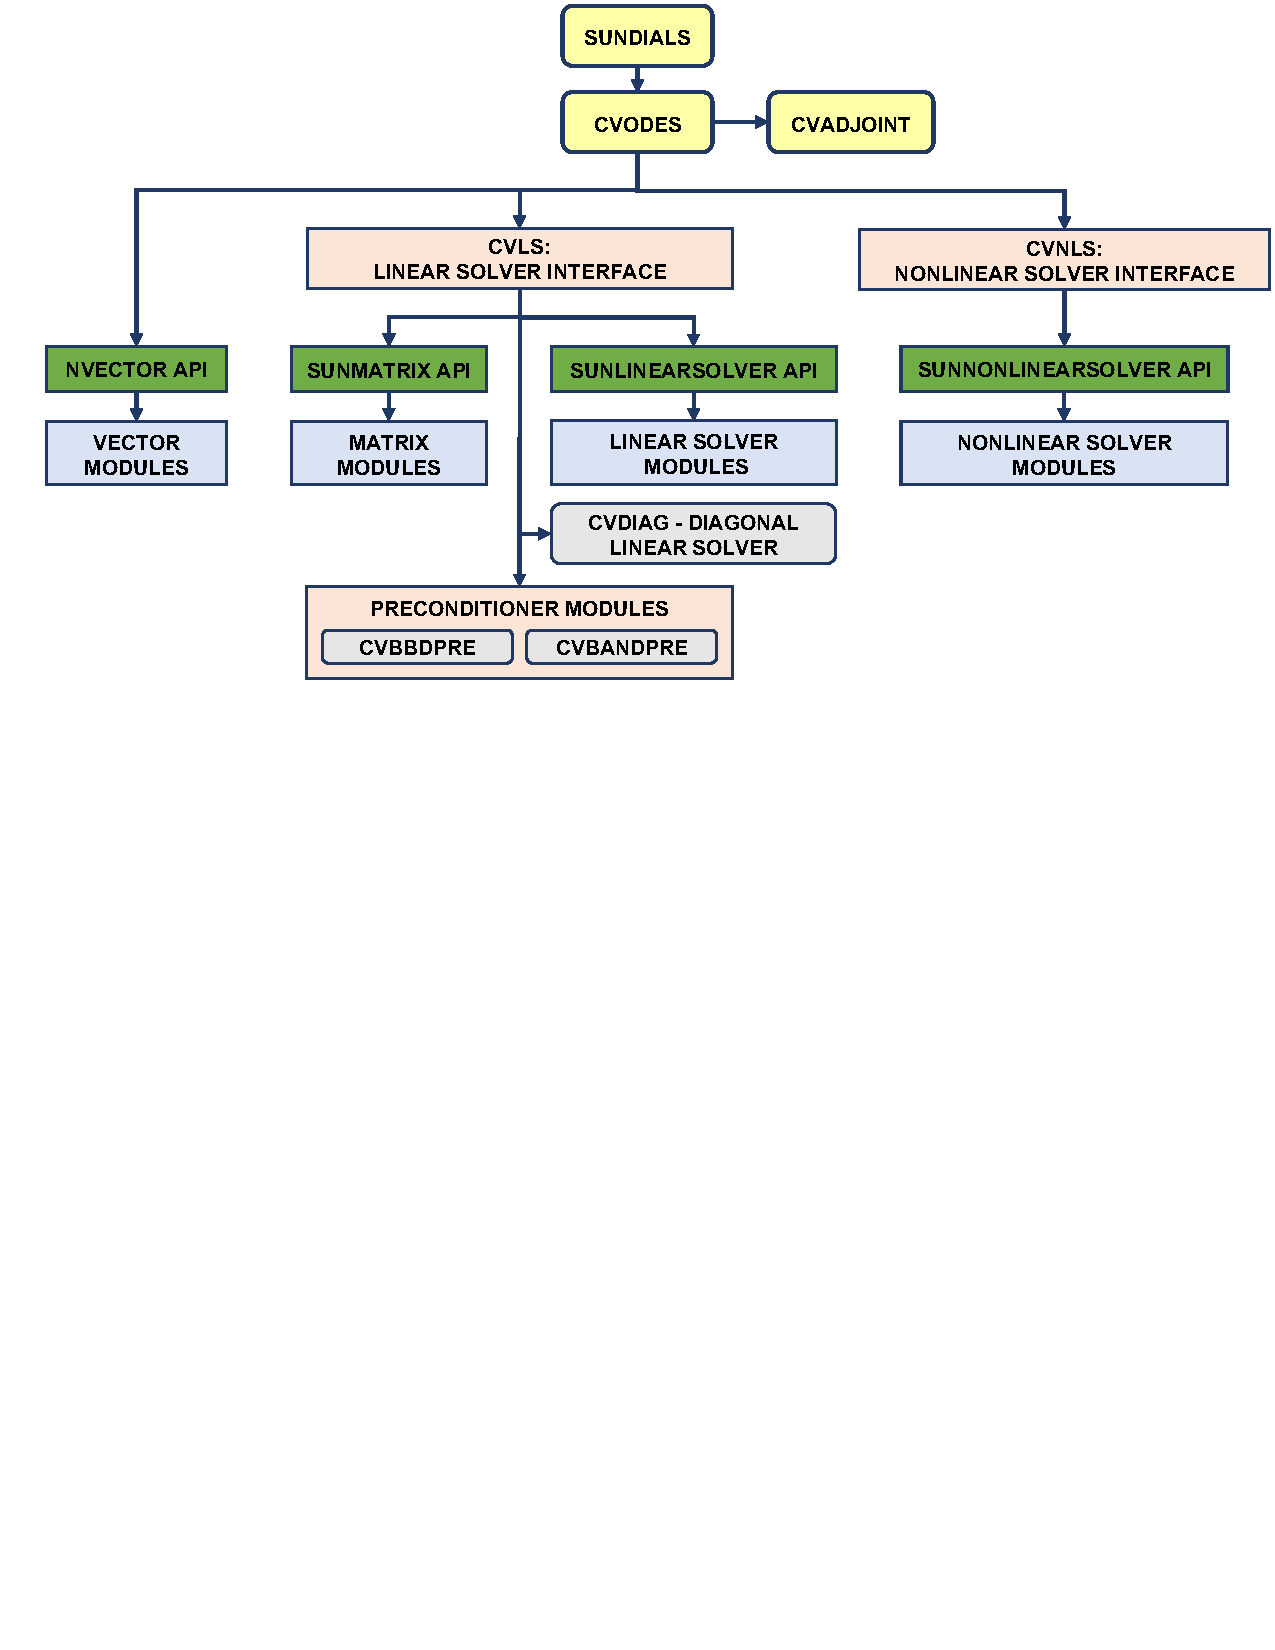
\includegraphics[width=\textwidth]{cvsorg}}}
\caption [Overall structure diagram of the {\cvodes} package]
{Overall structure diagram of the {\cvodes} package.
  Modules specific to {\cvodes} begin with ``CV'' ({\cvls}, {\cvdiag},
  {\cvbbdpre}, {\cvbandpre}, and {\cvnls}), all other items correspond
  to generic solver and auxiliary modules. 
  Note also that the LAPACK, {\klu} and {\superlumt} support is
  through interfaces to external packages.  Users will need to
  download and compile those packages independently.}
\label{f:cvsorg}
\end{figure}
The central integration module, implemented in the files \id{cvode.h},
\id{cvode\_impl.h}, and \id{cvode.c}, deals with the evaluation of integration
coefficients, estimation of local
error, selection of stepsize and order, and interpolation to user output
points, among other issues.

{\cvodes} utilizes generic linear and nonlinear solver modules defined by the
{\sunlinsol} API (see Chapter \ref{s:sunlinsol}) and {\sunnonlinsol} API (see
Chapter \ref{c:sunnonlinsol}), respectively. As such, {\cvodes} has no knowledge
of the method being used to solve the linear and nonlinear systems that
arise. For any given user problem, there exists a single nonlinear solver
interface and, if necessary, one of the linear system solver interfaces is
specified, and invoked as needed during the integration.

In addition, if forward sensitivity analysis is turned on, the main module 
will integrate the forward sensitivity equations simultaneously with the original
IVP. The sensitivity variables may be included in the local error control
mechanism of the main integrator.
\index{forward sensitivity analysis!correction strategies}
{\cvodes} provides three different strategies for dealing with the correction
stage for the sensitivity variables: \Id{CV\_SIMULTANEOUS}, \Id{CV\_STAGGERED} and
\Id{CV\_STAGGERED1} (see \S\ref{ss:fwd_sensi} and \S\ref{ss:sensi_malloc}).
The {\cvodes} package includes an algorithm for the approximation of the
sensitivity equations right-hand sides by difference quotients, but the user has
the option of supplying these right-hand sides directly.

\index{adjoint sensitivity analysis!implementation in {\cvodes}|(}
The adjoint sensitivity module (file \id{cvodea.c}) provides the infrastructure needed for the 
backward integration of any system of ODEs which depends on the solution 
of the original IVP, in particular the adjoint system and any quadratures required
in evaluating the gradient of the objective functional.  This module deals with
the setup of the checkpoints, the interpolation of the forward solution during
the backward integration, and the backward integration of the adjoint equations.
\index{adjoint sensitivity analysis!implementation in {\cvodes}|)}

\index{CVODES@{\cvodes} linear solver interfaces|(} 
At present, the package includes two linear solver interfaces.  The
primary linear solver interface, {\cvls}, supports both direct and
iterative linear solvers built using the generic {\sunlinsol} API (see
Chapter \ref{s:sunlinsol}).  These solvers may utilize a {\sunmatrix}
object (see Chapter \ref{s:sunmatrix}) for storing Jacobian
information, or they may be matrix-free. Since {\cvodes} can operate on
any valid {\sunlinsol} implementation, the set of linear solver
modules available to {\cvodes} will expand as new {\sunlinsol} modules
are developed.

Additionally, {\cvodes} includes the {\em diagonal} linear solver
interface, {\cvdiag}, that creates an internally generated diagonal
approximation to the Jacobian.
\index{CVODES@{\cvodes} linear solver interfaces|)} 

For users employing dense or banded Jacobian matrices, {\cvodes}
includes algorithms for their approximation through difference 
quotients, although the user also has the option of supplying a
routine to compute the Jacobian (or an approximation to it) directly.
This user-supplied routine is required when using sparse or
user-supplied Jacobian matrices.

For users employing matrix-free iterative linear solvers,
\index{Jacobian-vector product!setup and solve phases} {\cvodes}
includes an algorithm for the approximation by difference quotients of
the product $Mv$. Again, the user has the option of providing routines
for this operation, in two phases: setup (preprocessing of Jacobian
data) and multiplication. 

For preconditioned iterative methods, \index{preconditioning!setup and solve phases} 
the preconditioning must be supplied by the user, again in two phases: 
setup and solve.  While\index{preconditioning!advice on} there is no
default choice of preconditioner analogous to the difference-quotient
approximation in the direct case, the references
\cite{BrHi:89,Byr:92}, together with the example and demonstration
programs included with {\cvodes}, offer considerable assistance in
building preconditioners. 

\index{CVODES@{\cvodes} linear solvers!implementation details|(} 
{\cvodes}' linear solver interface consists of four primary phases,
devoted to (1) memory allocation and initialization, (2) setup of the
matrix data involved, (3) solution of the system, and (4) freeing of memory.  
The setup and solution phases are separate because the evaluation of
Jacobians and preconditioners is done only periodically during the
integration, and only as required to achieve convergence. 
\index{CVODES@{\cvodes} linear solvers!implementation details|)} 

{\cvodes} also provides two preconditioner modules, for use with any of
the Krylov iterative linear solvers. The first one, {\cvbandpre},
is intended to be used with {\nvecs}, {\nvecopenmp} or {\nvecpthreads}
and provides a banded difference-quotient Jacobian-based
preconditioner, with corresponding setup and solve routines.
The second preconditioner module, {\cvbbdpre}, works in conjunction
with {\nvecp} and generates a preconditioner that is a block-diagonal
matrix with each block being a banded matrix.

All state information used by {\cvodes} to solve a given problem is saved
in a structure, and a pointer to that structure is returned to the
user.  There is no global data in the {\cvodes} package, and so, in this
respect, it is reentrant. State information specific to the linear
solver is saved in a separate structure, a pointer to which resides in
the {\cvodes} memory structure. The reentrancy of {\cvodes} was motivated
by the anticipated multicomputer extension, but is also essential
in a uniprocessor setting where two or more problems are solved by
intermixed calls to the package from within a single user program.
